% Deutsche Parallelfassung zu geometry/curvature_transitions.tex

\chapter{Krümmungsübergänge}
\label{chap:curvature-transitions}

\section*{Motivation}

Das laufende Alignment hat die Grenze $s_1$ zwischen Gerade und
Übergangsbereich erreicht. Seine Krümmung muss null verlassen und bei $s_2$
die konstante Bogenkrümmung erreichen. Eine Koordinateninterpolation könnte
dieselben Endpositionen verbinden und dabei verbergen, wie sich Krümmung und
ihre Ableitungen an den Grenzen verhalten. Benötigt wird daher ein gesteuerter
Krümmungsübergangsprozess, der zu diesem identifizierten Alignment-Zustand
gehört.

\begin{principle}[Krümmungsübergangsprinzip]
\label{princ:curvature-transition}
Innerhalb von AIM ist ein Übergangsbogen primär ein Gesetz der
Krümmungsentwicklung, kein Interpolationsobjekt im Koordinatenraum.
\end{principle}

\section{Übergangsprinzip}

\begin{definition}[Krümmungsübergang]
\label{def:curvature-transition}
Ein Krümmungsübergang ist ein Krümmungsgesetz \(\kappa(s)\), das zwei
Krümmungszustände verbindet:
\[
\kappa_A\rightarrow\kappa_B.
\]
\end{definition}

Der Übergang bestimmt geometrische Glätte, dynamisches Verhalten,
Realisierungsstabilität, Laufzeitrobustheit und betrieblichen Komfort.

\begin{principle}[Übergangsprinzip]
\label{princ:transition-principle}
Innerhalb von AIM wird Übergangsgeometrie primär durch
Krümmungsentwicklung und nicht durch Koordinateninterpolation bestimmt.
\end{principle}

\section{Normierter Übergangsraum}

\begin{definition}[Normierter Übergangsparameter]
\label{def:normalized-transition-parameter}
Übergänge werden üblicherweise normiert auf
\[
w\in[0,1].
\]
\end{definition}

\begin{definition}[Normiertes Krümmungsgesetz]
\label{def:normalized-transition-law}
Ein normiertes Übergangsgesetz erfüllt
\[
\hat\kappa(w)\in[0,1].
\]
\end{definition}

Die Normierung trennt die intrinsische Übergangsform von der physischen
Skalierung. Dadurch werden wiederverwendbare Übergangsfamilien,
Familieninterpolation, Lookup-basierte Bewertung, normierte Optimierung und
kompakte dünn besetzte Repräsentation möglich.

Ein physischer Übergang entsteht durch Skalierung der normierten Krümmung und
Länge auf das tatsächliche Krümmungsintervall und die physische Bogenlänge.

\section{Übergangsfamilien}

\begin{definition}[Übergangsfamilie]
\label{def:transition-family}
Eine Übergangsfamilie ist eine Klasse normierter Krümmungsgesetze mit
gemeinsamen strukturellen Eigenschaften.
\end{definition}

Beispiele sind Klothoiden, polynomiale, trigonometrische, Bloss- und
Vienna-Übergänge sowie Lookup-basierte und hybride Übergangsfamilien. In AIM
werden sie als strukturierte Gebiete oder parametrisierte Pfade im normierten
Krümmungsraum interpretiert.

\section{Klothoidenübergang}

\begin{definition}[Klothoide]
\label{def:clothoid-transition}
Die Klothoide wird durch einen linearen Krümmungsverlauf definiert:
\[
\kappa(s)=a s+b.
\]
\end{definition}

In normierter Form entspricht sie \(\hat\kappa(w)=w\) und liefert einen
konstanten Krümmungsgradienten. Historisch wurde sie vorherrschend, weil sie
einfach, analytisch handhabbar, mit der klassischen Eisenbahnpraxis vereinbar
und dynamisch glatter als Krümmungssprünge ist.

In AIM ist die Klothoide nicht die universelle Übergangswahrheit, sondern ein
wichtiges Mitglied des Krümmungsübergangsraums.

\section{Polynomiale Übergänge}

\begin{definition}[Polynomialer Übergang]
\label{def:polynomial-transition}
Ein polynomialer Übergang erfüllt
\[
\kappa(s)=\sum_{i=0}^n a_i s^i.
\]
\end{definition}

Polynomiale Übergänge ermöglichen höhere Stetigkeit, Endpunkt- und
Ableitungsbedingungen sowie optimiertes dynamisches Verhalten. Sie sind
besonders nützlich, wenn Glattheitsbedingungen unmittelbar an
Krümmungsableitungen gestellt werden.

\section{Trigonometrische Übergänge}

\begin{definition}[Trigonometrischer Übergang]
\label{def:trigonometric-transition}
Ein trigonometrischer Übergang enthält sinus- oder kosinusbasierte
Krümmungsanteile.
\end{definition}

Diese Übergänge bieten häufig ein glatteres Verhalten höherer Ordnung als
Polynome niedrigen Grades und sind natürlich mit der spektralen Interpretation
des Krümmungsraums verbunden.

\section{Halbwelleninterpretation}

\begin{definition}[Halbwellenübergang]
\label{def:half-wave-transition}
Ein Halbwellenübergang ist ein normierter Krümmungsabschnitt, der
\[
0\rightarrow1
\quad\text{oder}\quad
1\rightarrow0
\]
verbindet.
\end{definition}

Innerhalb von AIM werden viele Übergangsfamilien kompositorisch interpretiert:
\[
\text{halfWave}_1\rightarrow\text{core}\rightarrow\text{halfWave}_2.
\]

Dies ermöglicht modulare Übergangskonstruktion, asymmetrische Übergänge,
Familieninterpolation und Übergangsdeformation. Die
Halbwelleninterpretation bietet eine gemeinsame Sprache zum Vergleich
klassischer und neu konstruierter Übergangsgesetze.

\section{Berlinish-Komposition}
\label{sec:berlinish-composition}

\emph{Berlinish} ist die im ursprünglichen Forschungsbeitrag verwendete
Bezeichnung für die verallgemeinerte Übergangskomposition
\[
T(s)
=
H_{\mathrm{in}}(s)
+
C(s)
+
H_{\mathrm{out}}(s).
\]
Dabei ist \(H_{\mathrm{in}}\) eine einlaufende Halbwelle, \(C\) ein
optionaler Klothoidenabschnitt und \(H_{\mathrm{out}}\) eine auslaufende
Halbwelle. Das Pluszeichen bezeichnet die geordnete stückweise Komposition auf
aufeinanderfolgenden Teilbereichen, nicht die Addition dreier überlagerter
Krümmungswerte. Jede Komponente darf die Länge null besitzen.

Für eine normierte Übergangskoordinate $w\in[0,1]$ sei die belegte Teilung
\[
\lambda=(\lambda_1,\lambda_c,\lambda_2),\qquad
\lambda_i\geq0,\qquad \lambda_1+\lambda_c+\lambda_2=1.
\]
Die gegenwärtige ausführbare Interpretation legt die Komponenten auf
\[
H_{\mathrm{in}}:[0,w_1],\qquad
C:[w_1,w_2],\qquad
H_{\mathrm{out}}:[w_2,1]
\]
mit
\begin{equation}
w_1=\lambda_1,qquad
w_2=\lambda_1+\lambda_c,qquad
\lambda=(w_1,w_2-w_1,1-w_2).
\label{eq:berlinish-partition-cuts}
\end{equation}
Damit sind $w_1,w_2$ in der gegenwärtigen Implementierung kumulierte
normierte Komponentenlängenanteile und Bereichsgrenzen. Bei einer physischen
Übergangslänge $L>0$ lauten die Komponentenlängen $L\lambda_i$. Die
Research-Evidenz stützt diese heutige Bedeutung, aber nur mit mittlerer
Sicherheit die Behauptung, dass die historische Berlinish-Quelle dieselben
Symbole verwendete. Heute sind sie editierbare Teilungsvariablen; die aktuelle
beschränkte AXTRAN-Optimierung begründet keine allgemeine Lösung für sie.

Diese eine Grammatik umfasst wichtige Grenzfälle:
\begin{itemize}
\item \(L_{H_{\mathrm{in}}}=L_{H_{\mathrm{out}}}=0\) ergibt eine reine
Klothoide;
\item \(L_C=0\) ergibt eine rein gekrümmte oder geglättete
Halbwellenkomposition;
\item eine Halbwelle der Länge null ergibt eine einseitige Komposition;
\item ungleiche Komponentenlängen oder verschiedene Halbwellenfunktionen
ergeben asymmetrische Übergänge;
\item positive Längen aller drei Komponenten ergeben zusammengesetzte
Übergänge.
\end{itemize}

Eine normierte Komponentenlänge null entfernt eine Komponente aus dieser
Komposition. Dies ist nicht derselbe Fall wie ein physisches Übergangselement
mit Gesamtlänge (L=0), bei dem kein Längsbereich verbleibt. Die getrennte
Behandlung verhindert, dass eine gültige reine Klothoidenteilung mit einem
physischen Null-Längen-Element verwechselt wird.

Polynomiale, trigonometrische und gemischte Funktionsfamilien können die
Halbwellen bilden. Ihr Verhalten wird nicht nur anhand von \(\kappa(s)\),
sondern auch anhand von
\[
\kappa'(s),\qquad \kappa''(s)
\]
verglichen, weil Endbedingungen und Verhalten höherer Ordnung Formen
unterscheiden, die visuell ähnliche Mittellinien erzeugen können. So lassen
sich etablierte nationale, historische oder proprietäre Übergangsformen in
einem gemeinsamen Vergleichsrahmen interpretieren, ohne ihre Namen oder ihre
Provenienz zu verlieren.

Vier Ebenen müssen getrennt bleiben. Die \emph{Funktionsidentität} bestimmt,
welches polynomiale, trigonometrische oder gemischte Gesetz verwendet wird.
Die \emph{Parametrisierung} bestimmt Skalierung und Teilung dieses Gesetzes.
Die \emph{Randbedingungen} bestimmen Krümmungen, Ableitungen,
Pose-Bedingungen und verfügbare Längen, die ein konkreter Anschluss erfüllen
muss. Die \emph{instanziierte Übergangsgeometrie} ist das berechnete Ergebnis,
nachdem diese Festlegungen gelöst und integriert wurden. Eine Familie ist
daher kein Alignment-Element, und eine gezeichnete Kurve ist nicht die
Familiendefinition.

\begin{figure}[ht]
\centering
\resizebox{\textwidth}{!}{% figures/geometry/berlinish_composition-DE.tex
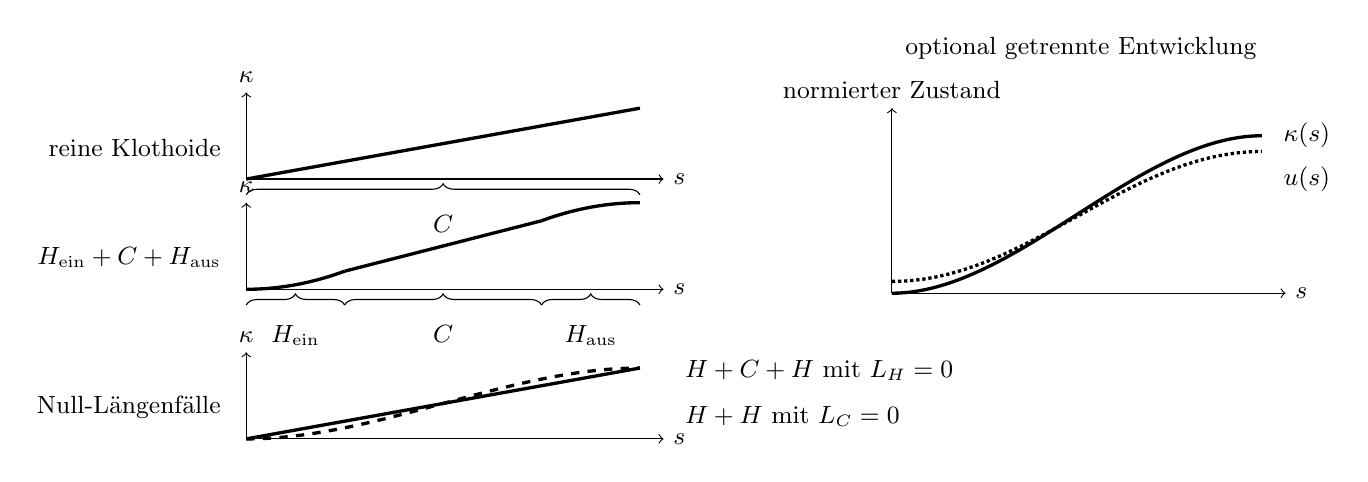
\begin{tikzpicture}[
  x=1cm,y=1cm,
  font=\small,
  axis/.style={->,thin},
  curve/.style={very thick},
  soft/.style={very thick,dashed},
  cant/.style={very thick,densely dotted},
  brace/.style={decorate,decoration={brace,amplitude=4pt}}
]
  \node[anchor=east] at (-0.2,3.75) {reine Klothoide};
  \draw[axis] (0,3.35) -- (5.3,3.35) node[right] {$s$};
  \draw[axis] (0,3.35) -- (0,4.45) node[above] {$\kappa$};
  \draw[curve] (0,3.35) -- (5,4.25);
  \draw[brace] (0,3.15) -- node[below=4pt] {$C$} (5,3.15);

  \node[anchor=east] at (-0.2,2.35) {$H_{\mathrm{ein}}+C+H_{\mathrm{aus}}$};
  \draw[axis] (0,1.95) -- (5.3,1.95) node[right] {$s$};
  \draw[axis] (0,1.95) -- (0,3.05) node[above] {$\kappa$};
  \draw[curve] plot[smooth,domain=0:1.25,samples=30] (\x,{1.95+0.23*(\x/1.25)^2});
  \draw[curve] (1.25,2.18) -- (3.75,2.82);
  \draw[curve] plot[smooth,domain=3.75:5,samples=30] (\x,{3.05-0.23*((5-\x)/1.25)^2});
  \draw[brace] (0,1.75) -- node[below=4pt] {$H_{\mathrm{ein}}$} (1.25,1.75);
  \draw[brace] (1.25,1.75) -- node[below=4pt] {$C$} (3.75,1.75);
  \draw[brace] (3.75,1.75) -- node[below=4pt] {$H_{\mathrm{aus}}$} (5,1.75);

  \node[anchor=east] at (-0.2,0.45) {Null-Längenfälle};
  \draw[axis] (0,0.05) -- (5.3,0.05) node[right] {$s$};
  \draw[axis] (0,0.05) -- (0,1.15) node[above] {$\kappa$};
  \draw[soft] plot[smooth,domain=0:5,samples=60] (\x,{0.05+0.9*(3*(\x/5)^2-2*(\x/5)^3)});
  \draw[curve] (0,0.05) -- (5,0.95);
  \node[anchor=west] at (5.45,0.92) {$H+C+H$ mit $L_H=0$};
  \node[anchor=west] at (5.45,0.33) {$H+H$ mit $L_C=0$};

  \begin{scope}[shift={(8.2,1.9)}]
    \node[anchor=south] at (2.4,2.85) {optional getrennte Entwicklung};
    \draw[axis] (0,0) -- (5.0,0) node[right] {$s$};
    \draw[axis] (0,0) -- (0,2.35) node[above] {normierter Zustand};
    \draw[curve] plot[smooth,domain=0:4.7,samples=60] (\x,{2.0*(3*(\x/4.7)^2-2*(\x/4.7)^3)});
    \draw[cant] plot[smooth,domain=0:4.7,samples=60] (\x,{0.15+1.65*(0.5-0.5*cos(180*\x/4.7))});
    \node[anchor=west] at (4.85,2.0) {$\kappa(s)$};
    \node[anchor=west] at (4.85,1.45) {$u(s)$};
  \end{scope}
\end{tikzpicture}
}
\caption{Berlinish-Vergleich: reine Klothoide, Halbwelle--Klothoide--Halbwelle-Komposition, Null-Längenfälle und optionale Trennung von Krümmungs- und Überhöhungsentwicklung.}
\label{fig:berlinish-composition}
\end{figure}

Der untere Vergleich in \cref{fig:berlinish-composition} macht einen weiteren
Freiheitsgrad ausdrücklich. Krümmung \(\kappa(s)\) beschreibt die Änderung der
Planrichtung je intrinsischer Länge; Überhöhung \(u(s)\) beschreibt den
Querneigungs- oder Schienenhöhenzustand unter der angegebenen Konvention.
Geschwindigkeit macht ihre gemeinsame Entwicklung betrieblich folgenreich,
doch sie sind nicht dieselbe Ingenieurgröße. Sie dürfen verschiedene
Funktionsinstanzen, Bereiche, physische Skalierungen, Teilungen,
Randbedingungen, Einheiten und Provenienz besitzen. Optionale Kopplung ist
eine Nebenbedingung zwischen den Gesetzen, nicht ihre Identität.

Die gegenwärtige Transition-Registry und der Evaluator implementieren nur
Krümmung; sie begründen weder einen Überhöhungsgesetz-Datensatz noch einen
validierten gemeinsamen Krümmungs--Überhöhungs-Optimierer. Historische
Vienna-Beispiele zeigen, warum Überhöhungsableitungen in eine gekoppelte
dynamische Beziehung eingehen können. Die überlieferte Evidenz wählt jedoch
weder eine autoritative moderne Kopplungsgleichung noch ein entsprechendes
Ziel. Gemeinsame Optimierung und eine einzelne kanonische Kopplung bleiben
daher Research und keine etablierte AIM-Fähigkeit.

\begin{remark}[Autorität der Bezeichnung Berlinish]
Berlinish bezeichnet in dieser Thesis einen ursprünglichen Forschungsbeitrag
und ein mathematisches Framework. Seine Komponenteninterpretation ist in der
aktuellen Transition-Registry implementiert; die Bezeichnung selbst wird
jedoch nicht als genehmigter Begriff des Knowledge Kernel behauptet.
\end{remark}

\section{Krümmungsanker}

\begin{definition}[Krümmungsanker]
\label{def:curvature-anchors}
Normierte Übergangsfamilien können die Ankerwerte
\[
0,\quad c_1,\quad c_2,\quad 1
\]
definieren.
\end{definition}

Anker beschreiben Übergangsteilung, Stetigkeitsbedingungen,
Normierungsstruktur und Familienkomposition. Mit ihnen lassen sich
Übergangsfamilien nach ihrer inneren Krümmungsstruktur statt nach ihrem
äußeren Erscheinungsbild im Positionsraum vergleichen.

\section{Übergangsstetigkeit}

\begin{definition}[Übergangsstetigkeit]
\label{def:transition-continuity}
Die Übergangsqualität hängt von der Stetigkeit von
\[
\kappa(s),\qquad \kappa'(s),\qquad \kappa''(s)
\]
ab.
\end{definition}

Höhere Stetigkeit verbessert Ruckverhalten, Realisierungsglätte,
Laufzeitstabilität, Fahrzeugreaktion und Fahrgastkomfort. Stetigkeit allein im
Positionsraum reicht zur Bewertung der Übergangsqualität nicht aus.

\section{Dünn besetzte Übergangsrepräsentation}

\begin{definition}[Dünn besetzter Übergang]
\label{def:sparse-transition}
Eine dünn besetzte Übergangsrepräsentation speichert Identität der
Übergangsfamilie, Normierungsparameter, Krümmungsanker,
Skalierungsparameter und Rekonstruktionsregeln.
\end{definition}

In AIM werden dünn besetzte Übergänge als kompakte Krümmungsoperatoren und
nicht als dichte geometrische Kurven interpretiert. Sie speichern, wie sich
Krümmung entwickeln soll, nicht eine abgetastete Polyliniennäherung der
resultierenden Geometrie.

\section{Lookup-basierte Übergänge}

\begin{definition}[Lookup-basierter Übergang]
\label{def:lookup-based-transition}
Ein Lookup-basierter Übergang verwendet abgetastete normierte Krümmung,
Interpolationsregeln, Ableitungsrekonstruktion und Laufzeitbewertung.
\end{definition}

Dies ermöglicht beliebige, experimentell entworfene,
realisierungsangepasste und fahrzeugspezifische Übergangsfamilien sowie
laufzeiteffiziente Bewertung. Lookup-basierte Übergänge sind kein Ersatz für
fehlende Theorie, sondern eine praktische Repräsentation von
Übergangsgesetzen im normierten Krümmungsraum.

\section{Übergangsableitungen}

\begin{definition}[Übergangsableitungen]
\label{def:transition-derivatives}
Wichtige Größen sind
\[
\kappa'(s),\qquad \kappa''(s),\qquad \kappa'''(s).
\]
\end{definition}

Sie beeinflussen Ruck, dynamische Glätte, Realisierungsverhalten,
Fahrzeugreaktion und Optimierungsstabilität. Das Ableitungsverhalten ist ein
wesentlicher Unterschied zwischen Übergangsfamilien, die im Positionsraum
ähnlich erscheinen können.

\section{Übergangssymmetrie}

\begin{definition}[Symmetrischer Übergang]
\label{def:transition-symmetry}
Ein normierter Übergang ist symmetrisch, wenn sein Krümmungsverlauf bezüglich
der Mitte des Übergangsintervalls symmetrisch ist.
\end{definition}

\begin{definition}[Asymmetrischer Übergang]
\label{def:transition-asymmetry}
Ein Übergang ist asymmetrisch, wenn diese Symmetrie bewusst verletzt wird.
\end{definition}

Asymmetrische Übergänge können Realisierungsqualität, Fahrzeugdynamik,
Topologieanpassung oder die Erfüllung geometrischer Nebenbedingungen
verbessern. Symmetrie ist daher eine Klassifikationseigenschaft, keine
universelle Anforderung.

\section{Frequenzverhalten von Übergängen}

Übergänge können durch ihren Krümmungsinhalt spektral interpretiert werden.
Hochfrequentes Krümmungsverhalten beeinflusst
Realisierungsempfindlichkeit, Maschinenglättung, Messempfindlichkeit und
dynamische Rauheit.

\begin{proposition}[Spektrales Übergangsprinzip]
\label{prop:spectral-transition-principle}
Übergangsqualität hängt nicht nur von Krümmungsstetigkeit, sondern auch vom
spektralen Verhalten im Krümmungsraum ab.
\end{proposition}

Dies verbindet die Übergangstheorie unmittelbar mit realisierungsstabiler
Krümmung und Krümmungsbandbreite.

\section{Übergangsrealisierung}

Der entworfene Übergang ist nicht notwendig der physisch realisierte
Übergang. Realisierung kann sein Verhalten durch Abtastung, Maschinenantwort,
strukturelle Filterung, Schottermechanik, Messrückkopplung und Grenzen lokaler
Korrektur verändern.

Übergangsqualität muss daher sowohl im Zielkrümmungsraum als auch im erwarteten
realisierten Krümmungsraum bewertet werden.

\section{Übergangsoptimierung}

Innerhalb von AIM wirkt Optimierung primär auf Übergangsfamilien,
Normierungsstruktur, Übergangslängen, Krümmungsanker,
Ableitungsverhalten und Krümmungsverlauf. Sie wird damit primär als
Optimierung im Krümmungsübergangsraum statt im Positionsraum interpretiert.

Eine realisierungsbewusste Optimierung kann nicht nur das
Zielübergangsgesetz \(\kappa_{\mathrm{target}}\), sondern auch das erwartete
realisierte Übergangsgesetz optimieren:
\[
\kappa_{\mathrm{real}}
=
\mathcal R_{\kappa}(\kappa_{\mathrm{target}}).
\]

\section{Kanonische Interpretation}

\begin{proposition}
Übergangsbögen sind grundlegend Krümmungsübergangsgesetze.
\end{proposition}
\begin{proposition}
Innerhalb von AIM wird Übergangsgeometrie intrinsisch im Krümmungsraum
interpretiert.
\end{proposition}
\begin{proposition}
Dünn besetzte Übergangsmodelle repräsentieren kompakte Übergangsoperatoren
statt ausdrücklicher geometrischer Kurven.
\end{proposition}
\begin{proposition}
Übergangsqualität hängt von Krümmungsverlauf, Ableitungsverhalten,
Spektralinhalt, Laufzeitstabilität und Realisierungsverhalten ab.
\end{proposition}

\section{Verbindung zu AIM}

\begin{summary}
Krümmungsübergänge bilden den dynamischen geometrischen Kern von AIM. In
diesem Framework werden Übergänge als Krümmungsentwicklungsprozesse und dünn
besetzte Modelle als Übergangsoperatoren interpretiert. Der normierte
Übergangsraum ermöglicht wiederverwendbare Familien, die
Halbwellenzerlegung modulare Konstruktion und Lookup-basierte Gesetze
experimentellen sowie realisierungsbewussten Entwurf. Laufzeitsysteme
rekonstruieren Geometrie dynamisch aus der Krümmungsstruktur.

Diese Interpretation vereinigt Übergangstheorie, Krümmungsklassifikation,
Realisierungsverhalten, Laufzeitbewertung und Optimierung in einem
intrinsischen Krümmungs-Framework.
\end{summary}
